% =====================================================================
%  Neural Networks 2026 (FaMAF-UNC) - Assignment 1
%  Numerical simulation of the Izhikevich neuron model
%
%  English version of the submitted report
%  (../../grupo36_mariel_anachuri_camila_giolitto_martin_robins_tp1.pdf).
%  Sections I-IV are a translation of the submitted text, section by
%  section. Section V adds Part 2 of the assignment (optional): the
%  network of 1000 neurons, which was not part of the submitted report.
%
%  Every figure and number comes from ../../../notebooks/TP1_Izhikevich_EN.ipynb.
%  Compile with pdfLaTeX + BibTeX (REVTeX 4.2; in Overleaf: Recompile).
% =====================================================================
\documentclass[aps,pre,twocolumn,10pt,nofootinbib,floatfix]{revtex4-2}

\usepackage[utf8]{inputenc}
\usepackage[T1]{fontenc}
\usepackage{lmodern}
\usepackage{amsmath,amssymb}
\usepackage{graphicx}
\usepackage{bm}
\usepackage{hyperref}

\graphicspath{{figures/}}

\renewcommand{\figurename}{Figure}
\renewcommand{\tablename}{Table}
\renewcommand{\labelitemi}{\scriptsize$\blacksquare$}

\makeatletter
\def\frontmatter@affiliationfont{\small}
\makeatother
\def\bibsection{\section*{\refname}}
\raggedbottom

\begin{document}

\title{Numerical simulation of the Izhikevich neuron model}

\author{Mariel Anachuri, Camila Giolitto, Martín Robins}
\affiliation{\mbox{Facultad de Matemática, Astronomía, Física y Computación, Universidad Nacional de Córdoba}\\
Neural Networks 2026}

\begin{abstract}
\textbf{Abstract.} The mathematical modelling of neurons requires balancing the realism of
the description with the simplicity needed for analysis and simulation. The Izhikevich model
lies at that middle point, since with two differential equations and four parameters it
reproduces a wide variety of firing patterns at a low computational cost. In this work, this
model was implemented and analysed, integrated with the fourth-order Runge--Kutta method (RK4)
with step $h = 0.1$ ms and a reset condition applied when $v \geq 30$ mV. First, the response
of a neuron with typical parameters to a current step was studied. Then, eight patterns of
neuronal activity were reproduced (RS, IB, CH, FS, LTS, TC1, TC2 and RZ). The simulations
qualitatively reproduce the patterns of the original paper and show that their diversity
depends on both the model parameters and the input current. Finally, the effect of the
integration step was analysed. Spike times depend on $h$ and their error accumulates with each
spike because of the reset, although the qualitative patterns are not altered. In an optional
second part, the 1000-neuron network program of the original paper was translated into Python:
it shows asynchronous activity at $\approx 7.8$ Hz with episodes of synchronisation, and
removing the self-connections does not change the collective dynamics.

\smallskip
\noindent{\footnotesize\textbf{Keywords:} Izhikevich model, numerical simulation, differential
equations, neuronal dynamics}
\end{abstract}

\maketitle

% =====================================================================
\section{Introduction}

Mathematical and computational modelling is a fundamental tool for studying how the nervous
system works, since it makes it possible to describe neuronal activity and to explore the
mechanisms that underlie it. As Dayan and Abbott~\cite{dayan2001} point out, a more detailed
model is not necessarily better; rather, it should act as a bridge between different levels
of understanding, incorporating enough information to represent the biological mechanisms of
interest while keeping the simplicity needed to facilitate its analysis.

This balance between detail and simplicity is reflected in spiking neuron models, which
describe the evolution of the membrane potential and the generation of action potentials in
response to input currents. Integrate-and-Fire models, derived from Lapicque's
proposal~\cite{lapicque1907}, represent the integration of the input currents and the firing
by means of a threshold, followed by a reset of the membrane potential, without describing the
action potential in detail. This facilitates mathematical analysis and reduces the
computational cost of simulations~\cite{dayan2001}. The Hodgkin--Huxley model, on the other
hand, incorporates voltage-dependent sodium and potassium conductances, which makes it
possible to describe the generation and time course of the action potential, although it
requires solving a more complex system of equations~\cite{hodgkin1952}.

In this context, the Izhikevich model combines the richness of neuronal dynamics that
characterises the Hodgkin--Huxley model with the computational efficiency of
Integrate-and-Fire models. Its formulation is based on bifurcation theory and on the reduction
to normal forms, which makes it possible to preserve relevant features of neuronal dynamics
through a simplified description. With two differential equations and a reset rule, it
reproduces different firing and bursting patterns by tuning four parameters, which
facilitates the simulation of large neural networks~\cite{izhikevich2003}.

The aim of this work is to study the ability of the Izhikevich model to reproduce different
patterns of neuronal activity through a simplified mathematical description. To this end, the
model was simulated with the fourth-order Runge-Kutta method, the way in which the parameters
and the input currents determine neuronal behaviour was analysed, the patterns obtained were
compared with those of the original paper, and the effect of the integration step on spike
times was evaluated.

% =====================================================================
\section{Theory and numerical methods}

\subsection{The Izhikevich model}

The model is described by the following system of two ordinary differential equations (ODEs):
\begin{align}
  \frac{dv}{dt} &= 0.04\,v^{2} + 5v + 140 - u + I, \label{eq:v}\\
  \frac{du}{dt} &= a\,(bv - u), \label{eq:u}
\end{align}
together with an after-spike reset mechanism:
\begin{equation}
  \text{if } v \geq 30~\text{mV, then}
  \begin{cases}
    v \leftarrow c,\\
    u \leftarrow u + d.
  \end{cases}
  \label{eq:reset}
\end{equation}
In these equations, time $t$ is measured in milliseconds (ms) and the membrane potential $v$
in millivolts (mV).

\subsection{Interpretation of the variables and the parameters}

The dynamics of the model is described by two state variables, an input current and four
parameters that regulate neuronal behaviour~\cite{izhikevich2003}.
\begin{itemize}
  \item $v$ \emph{(Membrane potential):} corresponds to the electrical potential difference
  across the membrane of the neuron and is expressed in millivolts (mV).
  \item $u$ \emph{(Recovery variable):} summarises the activation of potassium (K$^{+}$)
  currents and the inactivation of sodium (Na$^{+}$) currents. It provides negative feedback
  on the membrane potential.
  \item $I$ \emph{(Input current):} represents the current applied to the neuron, which may be
  injected directly or correspond to synaptic currents. In this work it is a function of time,
  and its versions $I_0$--$I_4$ are defined in Table~\ref{tab:cases}.
  \item $a$ \emph{(Time scale of $u$):} determines how fast the recovery variable $u$ evolves.
  Smaller values produce slower recovery. A typical value is $a = 0.02$.
  \item $b$ \emph{(Sensitivity of $u$ to $v$):} describes how the variable $u$ responds to the
  subthreshold fluctuations of $v$. Larger values couple both variables more strongly and may
  favour subthreshold oscillations and low-threshold spiking. A typical value is $b = 0.2$.
  \item $c$ \emph{(Potential reset):} sets the value to which $v$ is reset after reaching the
  spike peak ($+30$\,mV). It is related to the action of fast-activating potassium
  conductances. A typical value is $c = -65$\,mV.
  \item $d$ \emph{(Recovery jump):} determines the instantaneous increment added to the
  variable $u$ after reaching the spike peak. It is related to slower sodium and potassium
  conductances. A typical value is $d = 2$.
\end{itemize}

\subsection{Cutoff condition and threshold}

The value of $+30$\,mV is not a fixed physiological firing threshold; it is used as a
reference to detect the peak of the action potential and to apply the reset condition.

Unlike traditional Integrate-and-Fire (IF) models, which usually use a fixed threshold, the
Izhikevich model has a dynamic effective firing threshold, which depends on the previous state
of $v$ and $u$ and can vary approximately between $-55$\,mV and
$-40$\,mV~\cite{izhikevich2003}.

\subsection{Diversity of firing patterns}

Through different combinations of the parameters, the model can reproduce firing patterns
characteristic of different types of cortical and thalamic neurons~\cite{izhikevich2003}.
These include the excitatory neurons Regular Spiking (RS), Intrinsically Bursting (IB) and
Chattering (CH); the inhibitory interneurons Fast Spiking (FS) and Low-Threshold Spiking
(LTS); the thalamo-cortical regimes of tonic firing (TC1) and rebound bursting (TC2); and the
Resonator pattern (RZ) (Figure~\ref{fig:planes}).

\begin{figure}[t]
  \centering
  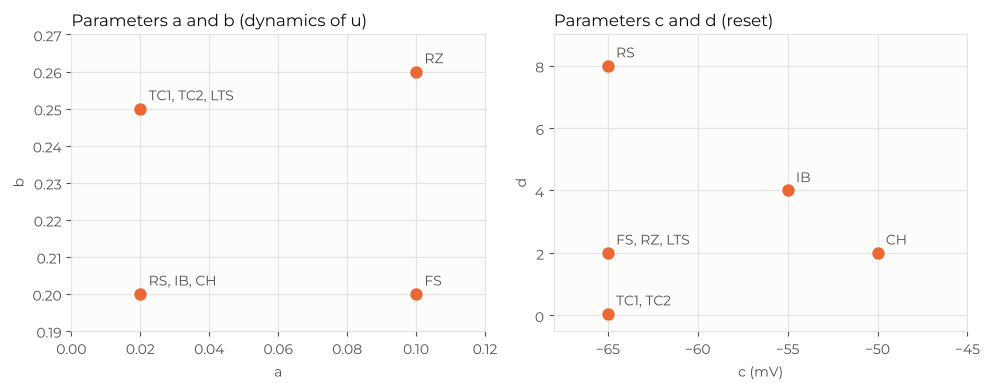
\includegraphics[width=\columnwidth]{fig1_parameter_space.png}
  \caption{Location of the eight configurations used in the parameter space of the Izhikevich
  model.}
  \label{fig:planes}
\end{figure}

\subsection{Numerical integration}

Equations~\eqref{eq:v} and~\eqref{eq:u} were integrated numerically with the fourth-order
Runge-Kutta method (RK4), implemented in Python, with an integration step of $h = 0.1$\,ms.
Given the state $\mathbf{x} = (v, u)$ at time $t$, the state at $t + h$ is computed as:
\begin{equation}
  \mathbf{x}(t + h) = \mathbf{x}(t) + \frac{h}{6}\left(\mathbf{k}_{1} + 2\mathbf{k}_{2}
  + 2\mathbf{k}_{3} + \mathbf{k}_{4}\right),
\end{equation}
where $\mathbf{k}_1, \dots, \mathbf{k}_4$ are evaluations of $\mathbf{f}$, the right-hand
side of Eqs.~\eqref{eq:v} and~\eqref{eq:u}, at the beginning, at two intermediate points and
at the end of each step.

After each integration step, it is checked whether $v \geq 30$\,mV; if so, the spike time is
recorded and the reset~\eqref{eq:reset} is applied immediately. For the figures, the point
$(t, 30\,\text{mV})$ is added at each spike before the reset value, since the integrator does
not store the peak.

The initial conditions were $u(0) = b\,v(0)$, with the values of $v(0)$ given in
Table~\ref{tab:cases}. The integration interval was $[0, 100]$\,ms for the base case and
$[0, 200]$\,ms for the patterns, except for RZ, whose interval was $[0, 300]$\,ms because its
pulse occurs at 180\,ms.

To evaluate the numerical error, the base case was repeated with $h = 0.2$, $0.05$ and
$0.01$\,ms, taking $h = 0.01$\,ms as the reference.

\begin{table*}[t]
  \caption{Parameters, initial potential and input current of the base case and of the eight
  simulated patterns. In all cases, $u(0) = b \cdot v(0)$.}
  \label{tab:cases}
  \begin{ruledtabular}
  \begin{tabular}{lcccccl}
    Case & $a$ & $b$ & $c$ (mV) & $d$ & $v(0)$ (mV) & Current ($t$ in ms) \\
    \hline
    Base case & 0.02 & 0.20 & $-65$ & 2    & $-70$   & $I_0$\; 0 ($t<10$); 10 ($t \geq 10$) \\
    RS        & 0.02 & 0.20 & $-65$ & 8    & $-65$   & $I_1$\; 0 ($t<20$); 10 ($t \geq 20$) \\
    IB        & 0.02 & 0.20 & $-55$ & 4    & $-65$   & $I_1$\; 0 ($t<20$); 10 ($t \geq 20$) \\
    CH        & 0.02 & 0.20 & $-50$ & 2    & $-65$   & $I_1$\; 0 ($t<20$); 10 ($t \geq 20$) \\
    FS        & 0.10 & 0.20 & $-65$ & 2    & $-65$   & $I_1$\; 0 ($t<20$); 10 ($t \geq 20$) \\
    TC1       & 0.02 & 0.25 & $-65$ & 0.05 & $-63$   & $I_2$\; 0 ($t<20$); 1 ($t \geq 20$) \\
    TC2       & 0.02 & 0.25 & $-65$ & 0.05 & $-65$   & $I_3$\; 0 ($t<20$); $-25$ ($20 \leq t < 80$); 0 ($t \geq 80$) \\
    RZ        & 0.10 & 0.26 & $-65$ & 2    & $-62.5$ & $I_4$\; 0 ($t<40$); 0.2 ($40 \leq t < 180$); 2.2 ($180 \leq t < 181$); 0.2 ($t \geq 181$) \\
    LTS       & 0.02 & 0.25 & $-65$ & 2    & $-65$   & $I_1$\; 0 ($t<20$); 10 ($t \geq 20$) \\
  \end{tabular}
  \end{ruledtabular}
\end{table*}

% =====================================================================
\section{Results}

\subsection{Neuronal response to a current step}

The response of the base case to a current step applied at $t = 10$\,ms was analysed first.
Figure~\ref{fig:base} shows the evolution of the membrane potential and of the recovery
variable, together with the input current. Until the stimulus is applied, the neuron remains
at rest ($v = -70$\,mV). A train of spikes is then observed, the first at $t = 13.5$\,ms,
whose intervals between consecutive spikes increase progressively from 3.6\,ms to about
19\,ms until an approximately periodic regime is reached. Each spike is accompanied by an
increment of $u$ of value $d = 2$, followed by a slow relaxation of $u$ until the next spike.
This accumulation of $u$ is what progressively lengthens the intervals between spikes.

\begin{figure}[b]
  \centering
  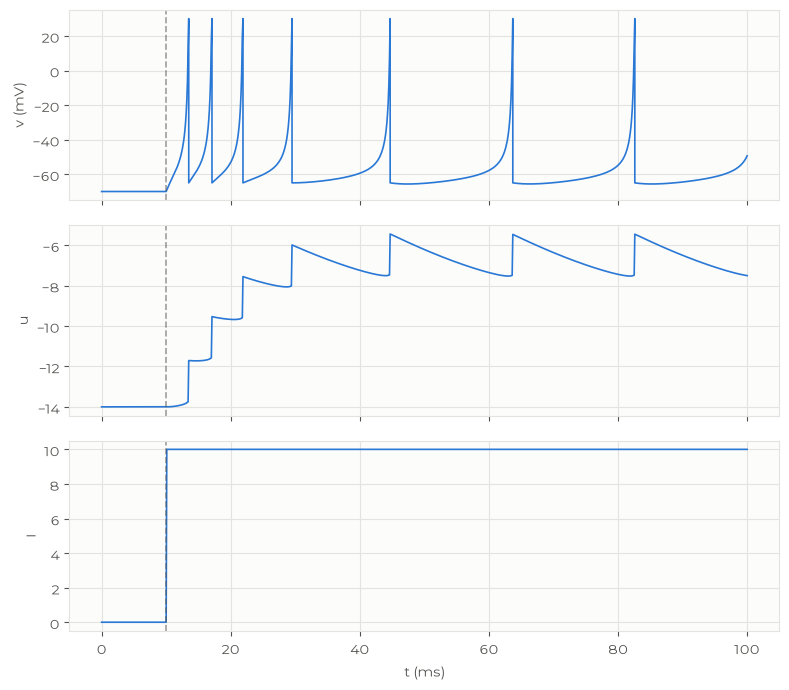
\includegraphics[width=\columnwidth]{fig2_base_case.png}
  \caption{Time evolution of the membrane potential $v(t)$, the recovery variable $u(t)$ and
  the input current $I(t)$ (from top to bottom).}
  \label{fig:base}
\end{figure}

\subsection{Neuronal dynamics for different configurations}

Figure~\ref{fig:eight} presents the response of the eight parameter configurations
corresponding to the different neuron types. RS, IB, CH, FS and LTS receive the same current
step ($I_1 = 10$) from 20\,ms onwards, so their different responses are due exclusively to the
change in the model parameters. RS, FS and LTS produce single spikes, with different
frequencies and time courses. RS fires at low frequency; after a shorter first interval, the
following ones become longer and keep a constant period. LTS, in contrast, starts firing at
high frequency and its intervals grow progressively until they stabilise. FS has the highest
frequency and keeps practically constant intervals throughout the stimulus. IB and CH, for
their part, respond with bursts. In IB there is an initial burst followed by isolated spikes
at regular intervals, whereas in CH the bursts repeat at approximately regular intervals
throughout the stimulus.

The thalamo-cortical neuron responds in two different ways depending on the stimulus it
receives. In TC1, a weak constant current makes the neuron fire one spike at a time, with
well-separated spikes. In TC2, the current is negative: while it is applied, the potential
drops below rest, and when it is removed, the neuron responds with a burst of spikes before
returning to rest.

Finally, in RZ a small current makes the potential oscillate slightly, but without firing.
Only when a brief pulse is applied at 180\,ms does the neuron start firing repetitively.

\begin{figure*}[t]
  \centering
  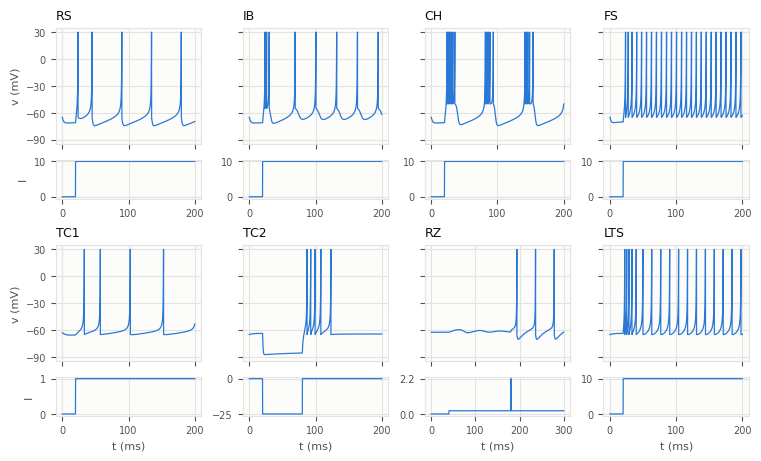
\includegraphics[width=0.82\textwidth]{fig3_eight_patterns.png}
  \caption{Membrane potential $v(t)$ and input current $I(t)$ (below each panel) for the eight
  patterns: RS, IB, CH, FS, TC1, TC2, RZ and LTS (parameters and currents in
  Table~\ref{tab:cases}).}
  \label{fig:eight}
\end{figure*}

\subsection{Effect of the integration step}

Figure~\ref{fig:error} shows the effect of the integration step on the base case. All four
steps produce seven spikes, but their times are shifted: with the largest step
($h = 0.2$\,ms) the spikes are delayed with respect to the reference. This difference grows
with the number of spikes, with a marked increase between the fourth and the fifth spike. At
the last spike, the shift is 2.5\,ms with $h = 0.2$\,ms, 0.7\,ms with $h = 0.1$\,ms and
0.3\,ms with $h = 0.05$\,ms.

\begin{figure}[t]
  \centering
  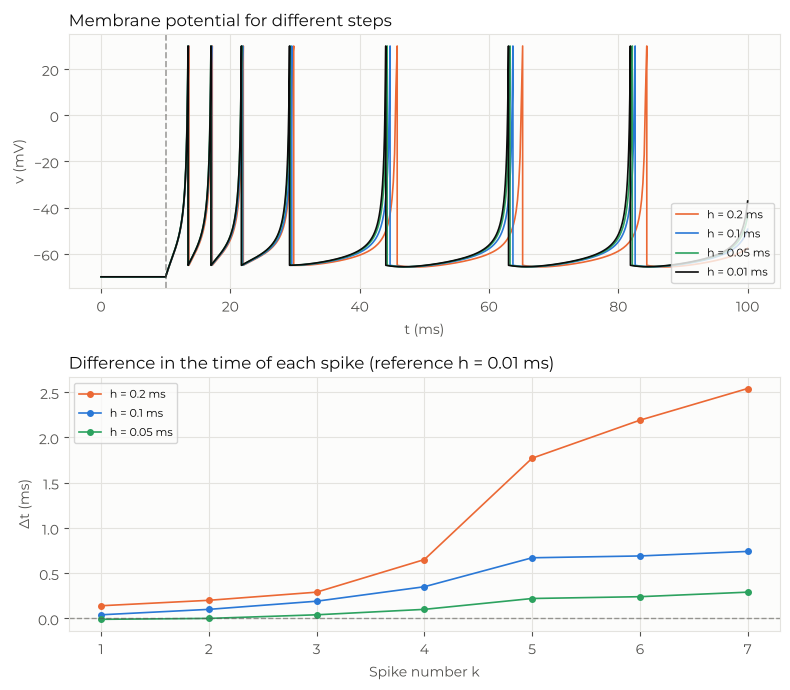
\includegraphics[width=0.8\columnwidth]{fig4_integration_step.png}
  \caption{Effect of the integration step on the base case. Top, membrane potential for
  $h = 0.2$, $0.1$, $0.05$ and $0.01$\,ms. Bottom, shift of each spike with respect to
  $h = 0.01$\,ms.}
  \label{fig:error}
\end{figure}

% =====================================================================
\section{Discussion and conclusions}

The simulations qualitatively reproduce the eight patterns of Figure~2 of
Izhikevich~\cite{izhikevich2003}, and their differences can be explained by how the parameters
regulate the brake that $u$ exerts on $v$. A large $d$ strengthens the brake with each spike
and produces adaptation (RS), a large $a$ releases it quickly and prevents adaptation (FS),
and a high $c$ leaves $v$ close to firing after the reset and generates bursts that repeat or
not depending on $d$ (CH and IB). In TC2, the negative current also reduces $u$, and when it is
removed the neuron is left with little brake and fires. RZ shows the bistability between rest
and repetitive firing described in the paper. Since the protocols of TC1, TC2 and RZ are
specific to this assignment, the comparison in those cases is qualitative, and they show that
the same neuron responds differently depending on the stimulus it receives.

In the numerical integration (Figure~\ref{fig:error}), the main source of error is the
reset. The spike is detected at the end of the step in which $v$ exceeds 30\,mV, with an error
of up to one step $h$, and since each spike starts from the previous reset, the shifts
accumulate. Thus, although RK4 is a fourth-order method, the reset limits the accuracy of the
spike times. With $h = 0.1$\,ms, the step used in the paper, the spike times depend on the
step, but the patterns are not altered.

In summary, with two differential equations and four parameters, the Izhikevich model
reproduces a wide variety of neuronal behaviours without describing in detail the mechanisms
that give rise to them. It thus lies at the middle point between detail and simplicity put
forward by Dayan and Abbott~\cite{dayan2001}, which makes it possible to simulate networks
with a large number of neurons~\cite{izhikevich2003}.

% =====================================================================
\section{Part 2 (optional): network of 1000 neurons}

In the optional second part of the assignment, the MATLAB program of Section~IV of
Ref.~\cite{izhikevich2003} was translated into Python and simulated, and two variants of it
were explored.

\begin{figure*}[t]
  \centering
  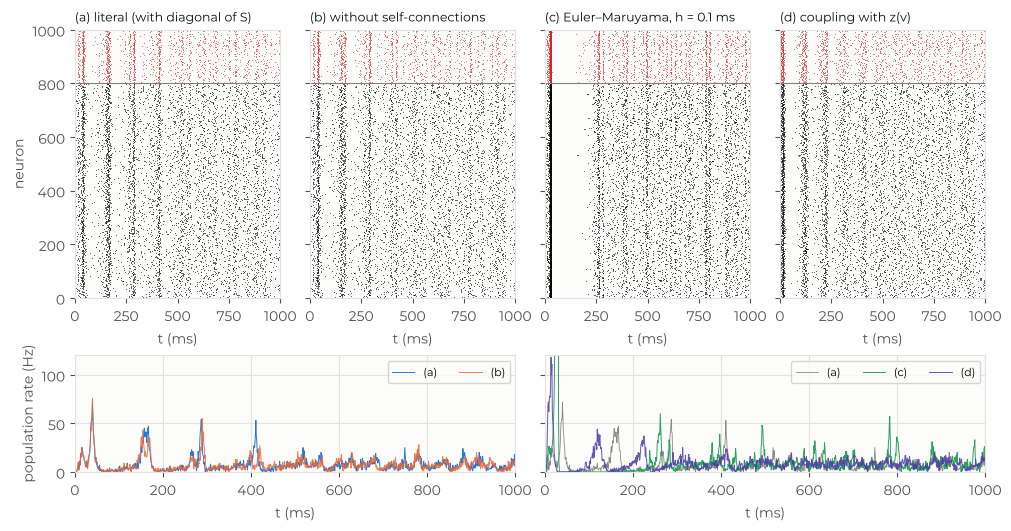
\includegraphics[width=0.92\textwidth]{fig5_network.png}
  \caption{Network of 1000 neurons during 1000\,ms (seed 2026). Top: raster plots (each dot is
  a spike; excitatory neurons 1--800 in black and inhibitory neurons 801--1000 in red) of
  (a) the literal translation of the paper's MATLAB code, (b) the same network with
  $s_{ii} = 0$, (c) the Euler--Maruyama variant and (d) the variant with continuous coupling
  $z(v)$. Bottom: population rate (spikes per neuron in 1\,ms bins, in Hz); on the left (a)
  and (b), on the right (a) in grey, (c) and (d).}
  \label{fig:network}
\end{figure*}

\subsection{Network model and numerical method}

The network has $N_e = 800$ excitatory and $N_i = 200$ inhibitory neurons governed by
Eqs.~\eqref{eq:v}--\eqref{eq:reset}, with heterogeneous parameters ($r_i \sim U(0,1)$):
$a_i = 0.02$, $b_i = 0.2$, $c_i = -65 + 15r_i^2$, $d_i = 8 - 6r_i^2$ for the excitatory
neurons (from RS to CH) and $a_i = 0.02 + 0.08r_i$, $b_i = 0.25 - 0.05r_i$, $c_i = -65$,
$d_i = 2$ for the inhibitory ones (from LTS to FS). The weights are
$S = [\,0.5R_E \mid -R_I\,]$, with $R_E$ and $R_I$ uniform in $[0,1]$ and $s_{ij}$ the weight
from neuron $j$ to neuron $i$. At each 1\,ms step the input is
$I_i = I_i^{\rm ext} + I_i^{\rm syn}$, with thalamic noise $I_i^{\rm ext} = 5\xi_i$
(excitatory) or $2\xi_i$ (inhibitory), $\xi_i \sim N(0,1)$, and pulse coupling
$I_i^{\rm syn} = \sum_{j \in F} s_{ij}$, where $F$ is the set of neurons that fired; $v$ is
updated with two Euler steps of 0.5\,ms and $u$ with one of 1\,ms. The matrix $S$ is dense and
its diagonal is not set to zero: there are self-connections $s_{ii} \neq 0$. All the
simulations start from $v = -65$\,mV, $u = b\,v$, last 1000\,ms and use the seed 2026.

\emph{Euler--Maruyama variant.} Between spikes,
$dV_i = (0.04V_i^2 + 5V_i + 140 - U_i)\,dt + \sigma_i\,dW_i$ and
$dU_i = a_i(b_iV_i - U_i)\,dt$, with $\sigma_i = 5$ or 2, keeping the synaptic jumps and the
reset separate, with step $h = 0.1$\,ms. The scheme is
$Y_{n+1} = Y_n + f(Y_n)\,h + \sigma\sqrt{h}\,\xi_n$~\cite{kloeden1992}: the Wiener increment
over a step $h$ has variance $h$, hence the factor $\sqrt{h}$. In the literal reproduction of
the MATLAB code this factor does not apply, because there the noise is a discrete current
drawn once per millisecond, not a Wiener process.

\emph{Variant with $z(v)$.} We propose replacing the pulse coupling with the continuous
current $I_i^{\rm syn}(t) = \sum_j s_{ij}\,z(v_j(t))$, with $z(v) = (87 + v)/450 - 0.0193$
and $v$ clipped at 30\,mV, leaving everything else unchanged. $z(v)$ is not a spike detector:
at rest it is $\approx 0.03$, so each neuron receives a permanent background input. It is a
different model from that of Figure~3 of Ref.~\cite{izhikevich2003}, and we use it only as a
comparative experiment.

\subsection{Results}

In Figure~\ref{fig:network}(a), asynchronous background activity is observed, interrupted by
episodes of synchronisation: vertical bands in which a large part of the population fires at
the same time, with peaks of the population rate at $\approx 40$, 160, 290 and 410\,ms. The
first one occurs at the start, with all the neurons at $v = -65$\,mV. After $\approx 450$\,ms
the bands are weaker. The literal network emits 7765 spikes, with a mean rate of 7.77\,Hz
(7.82\,Hz for the excitatory neurons and 7.57\,Hz for the inhibitory ones), and the spectrum
of the population rate for $t > 100$\,ms has its maximum at $\approx 7.8$\,Hz.

With the same seed and without self-connections [Figure~\ref{fig:network}(b)], the network
emits 7561 spikes (7.56\,Hz). The large episodes appear at similar times ($\approx 40$, 150,
290 and 400--420\,ms), with somewhat different amplitudes, while the individual spikes differ.
Repeating the comparison with 20 seeds ($t > 100$\,ms), the mean rate is
$7.19 \pm 0.13$\,Hz with the diagonal and $7.17 \pm 0.13$\,Hz without it; the difference is
$0.02 \pm 0.12$\,Hz.

In the Euler--Maruyama variant [Figure~\ref{fig:network}(c)] there is a very intense initial
episode between 3.5 and 33.4\,ms, in which each neuron fires about 24 times (24\,357 spikes),
followed by almost 200\,ms of near silence; then asynchronous activity with bands appears,
with a mean rate of 8.23\,Hz for $t > 100$\,ms. With continuous coupling $z(v)$
[Figure~\ref{fig:network}(d)] there is also an asynchronous background with bands, wider at
the beginning (8804 spikes; 8.35\,Hz for $t > 100$\,ms, compared with 7.54\,Hz for the
literal network over the same interval).

\subsection{Discussion}

The literal translation reproduces what the paper describes for its Figure~3: asynchronous
activity with mean rates of $\approx 8$\,Hz and occasional episodes of synchronisation. The
large episodes repeat every $\approx 120$\,ms, which matches the spectral maximum at
$\approx 7.8$\,Hz, close to the $\alpha$ band ($\approx 10$\,Hz) reported in the paper. The
self-connections contribute a single weight to each neuron (at most 0.5 if it is excitatory,
or down to $-1$ if it is inhibitory) against the sum of the inputs from the whole network:
removing them changes the individual spikes, but not the mean rate (the difference over
20 seeds is much smaller than its spread) nor the structure of the synchronous episodes. We
conclude that the diagonal of $S$ does not qualitatively modify the dynamics.

In the Euler--Maruyama variant, the synaptic jumps are applied every 0.1\,ms; we infer that,
with all the neurons starting from the same state, the first synchronous discharge generates
jumps that push $v$ above 30\,mV again in the following steps, which produces the initial
episode of $\approx 24$ spikes per neuron. Once this transient is over, the dynamics (rate
$\approx 8$\,Hz with bands) is comparable to that of the original. The variant with $z(v)$ is
a different model: the synaptic input does not depend on the firing events but on the
potential of all the neurons at all times, so it includes a permanent background that raises
the rate ($\approx 8.3$ versus $\approx 7.5$\,Hz) and changes the shape of the episodes; it
does not reproduce Figure~3 of the paper and serves only as a comparison.

% =====================================================================
\bibliography{references}

\end{document}
